\lstinputlisting[language=bash,basicstyle=\small]{python_codes/fieldstone_72/keywords}

\begin{center}
Code at \url{https://github.com/cedrict/fieldstone/tree/master/python_codes/fieldstone_72}
\end{center}

\par\noindent\rule{\textwidth}{0.4pt}

%%%%%%%%%%%%%%%%%%%%%%%%%%%%%%%%%%%%%%%%%%%%%%%%%%%%%%%%%%%%%%%%%%%%%%%%%%%%%%%%%%%%%%%%%%%%%%%%%%%%

\subsubsection*{Manufactured solution}

The analytical solution originates in Lamichhane (2015) \cite{lami15} and is 
presented in Section~\ref{ss:mms11}. 
The quadrilateral MINI element used here also originates in the same article 
and comes in two flavours with two different bubble functions $b_1$ and $b_2$
as explained in Section~\ref{ss:quadmini}.
The velocity and pressure fields are shown hereunder:

\begin{center}
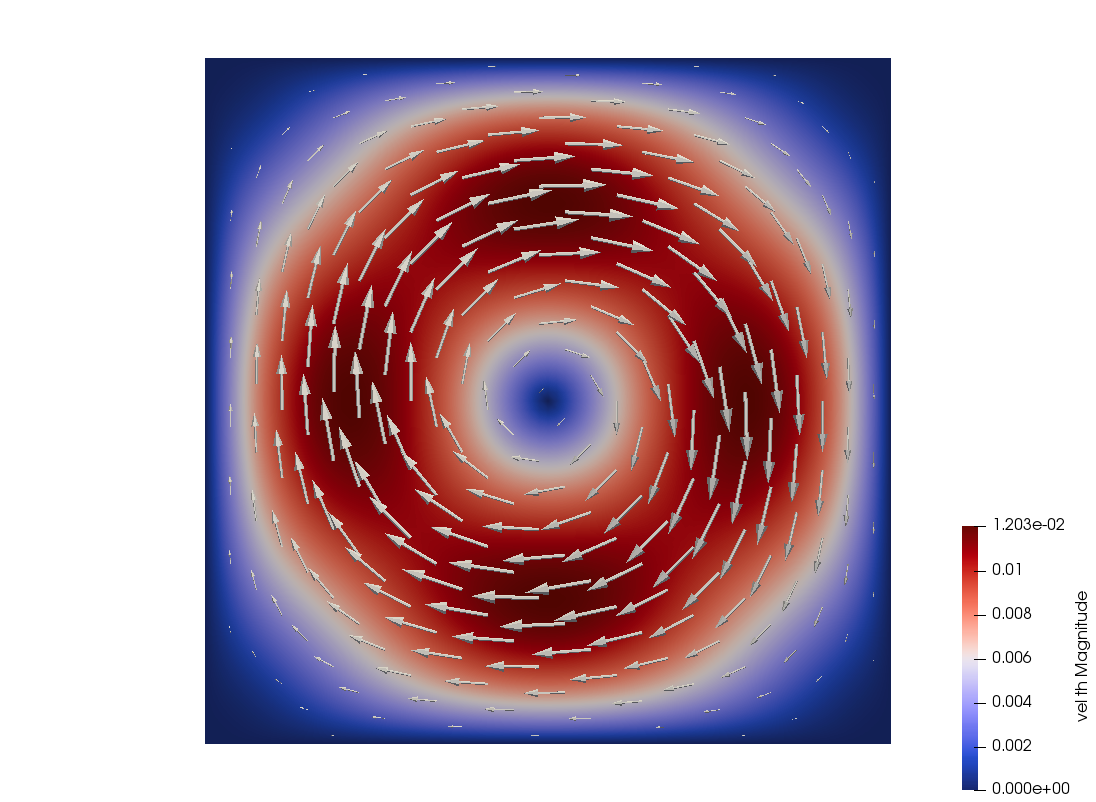
\includegraphics[width=7cm]{python_codes/fieldstone_72/results/mms/vel}
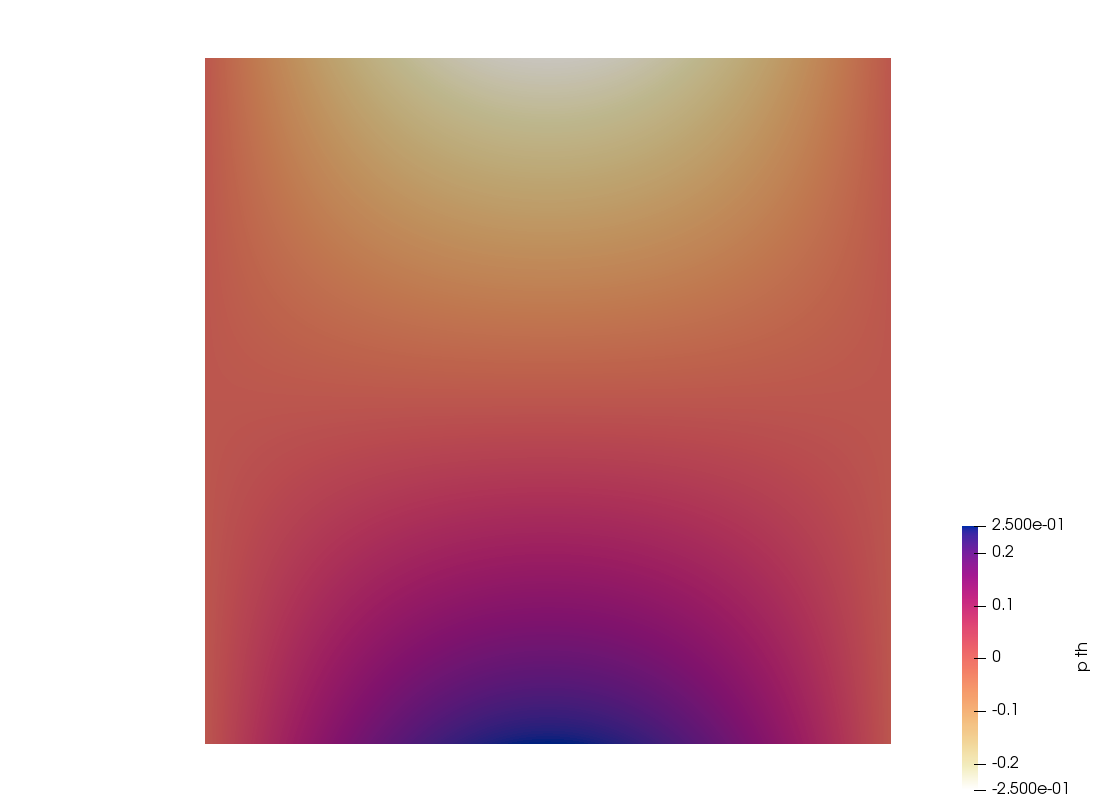
\includegraphics[width=7cm]{python_codes/fieldstone_72/results/mms/p}
\end{center}

During the debugging process I ended up 
implementing various quadratures, from $2^2$ to $6^2$ points. 
The results from the article are different than mine but I suspect that what the 
author measured could be different than what I measure. 
The trends are similar with $b_2$ performing better than $b_1$ (and 
we also observe that the quadrature scheme does not alter results at all): 

\begin{center}
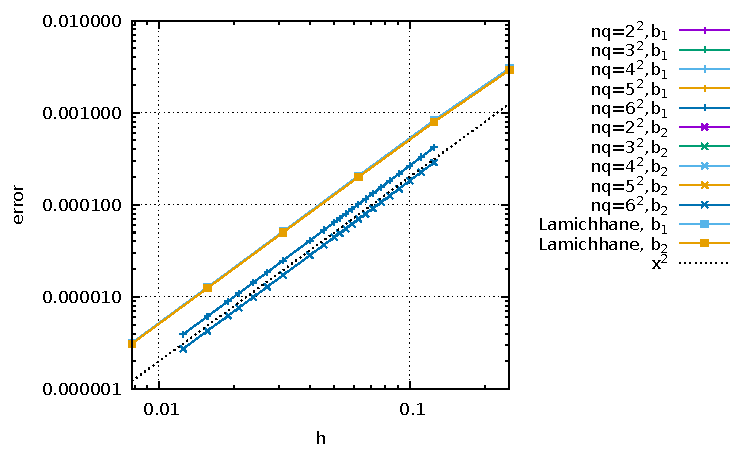
\includegraphics[width=7cm]{python_codes/fieldstone_72/results/mms/errors_v}
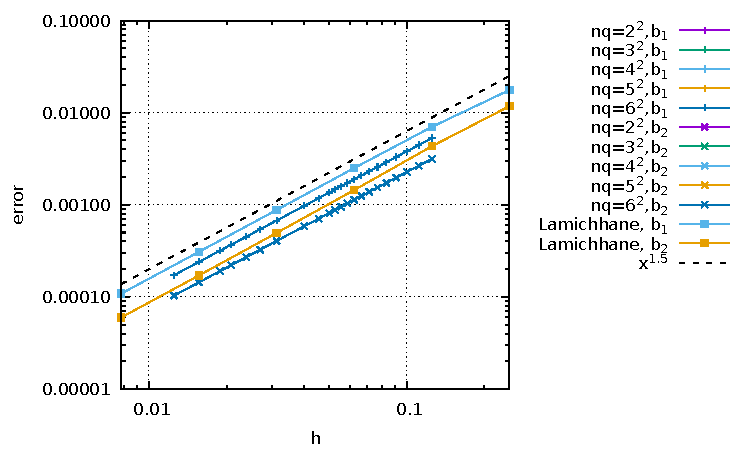
\includegraphics[width=7cm]{python_codes/fieldstone_72/results/mms/errors_p}\\
{\captionfont Left: velocity error in $L_2$ norm; Right: pressure error in $L_2$ norm.\\
Resolutions from $8\times8$ until $80\times80$.}
\end{center}

The root mean square velocity is also measured for both bubble functions.
As above we see that $b_2$ performs better than $b_1$:
\begin{center}
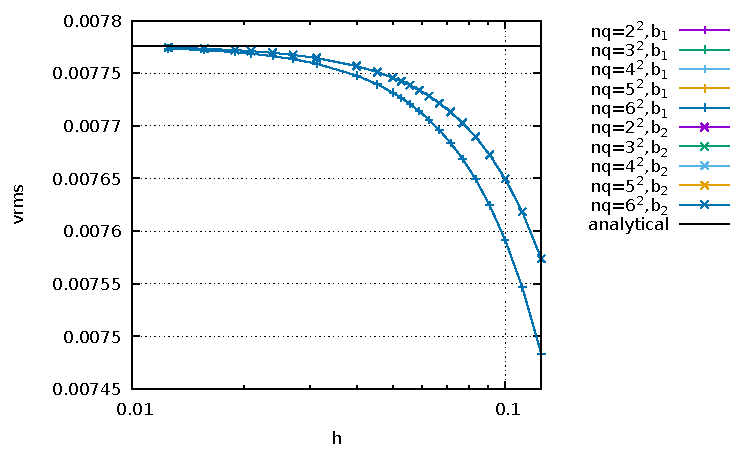
\includegraphics[width=10cm]{python_codes/fieldstone_72/results/mms/vrms}
\end{center}



